
%%%%%%%%%%%%%%%%%%%%%%%%%%%%%%%%%%%%%%%%%%%%%%%%%%%%%%%%%%%%%%%%%%%%%%%%%%%%%%%%
%%%%%%%%%%%%%%%%%%%%%%%%%%%%%%%%%%%%%%%%%%%%%%%%%%%%%%%%%%%%%%%%%%%%%%%%%%%%%%%%
\section{Dançando no tempo forte e em contratempo}
\index{Musicalidade!Dançando no tempo forte}
\index{Musicalidade!Dançando em contratempo}

Nesta seção será proposto um modo de uso da palavra 
\hyperref[sec:contratempo]{\textbf{contratempo}} no contexto da dança;
este uso estará de acordo com o já achado na literatura  sobre dança,
e a definição de tempo e contratempo na literatura sobre música.

\subsection{Tempo forte e contratempo na dança espanhola}
\label{subsec:contratempoespanha}
No livro sobre dança espanhola, ``Compendio de las principales reglas del baile'' (1820) \cite[pp. 131]{cairon1820compendio},
podemos ver a descrição de passos denominados contratempos.
\begin{citando}
Se llaman \textbf{contratiempos} todos aquellos pasos en que estando colocado el cuerpo sobre un pie,
y teniendo el otro en el aire,
se salta sobre el que está en el suelo antes de colocar el otro en tierra;
\end{citando}
Assim, na dança espanhola de 1820 são conhecidos como contratempos,
movimentos em que se impulsa ou salta num pé e se pisa com o outro. 
A relação dos passos com pulos, na dança espanhola, 
com o contratempo na música, 
é explicado na tésis de doutorado titulada 
``La danza en España en la segunda mitad del siglo XVIII: El bolero'' (2017)
\cite[pp. 160]{martin2017danza} onde se menciona:
\begin{citando}
En el Amable de estilo italiano se ejecutaban pasos saltados muy complicados como el sisone,
asamblé, jeté, piruetas y diversidad de saltos executados en los \textbf{contratempos} musicales.
\end{citando}
É dizer, os passos pulados eram executados nos contratempos musicais;
ou seja, acentuando mais o tempo fraco que o tempo forte,
ou acentuando mais a parte fraca do tempo que a parte forte deste;
de modo que estes saltos foram denominados a contratempo.
Podemos ver esta relação no livro ``Glosario de términos de la danza española'' (2001)
\cite[pp. 109]{aubero2001glosario}, onde mencionam:
\begin{citando}
Despues del <<salto mayor>>, cuando el bailarín salta en el aire en el $4^o$ tiempo,
puede caer sobre ambos pies juntos (a pie) o en <<contratiempo>>.
\end{citando}
Confirmando-nos que o pulo era feito num tempo fraco (quarto tempo).



\subsection{Tempo forte e contratempo na dança em cuba}
\label{subsec:contratempocuba}
No ``Diccionario de la música cubana'' (1981) 
\cite[pp. 113]{orovio1981diccionario} \cite[pp. 57]{santana2005merengue},
podemos achar o seguinte texto relativo às palavras do compositor e músico Enrique Jorrín.
\begin{citando}
Noté la dificultad de la mayoría en los ritmos sincopados, 
debido a que los pasos de los bailadores se producen a \textbf{contratiempo},
o sea en la segunda y cuarta corchea del compás de dos quartos.
\end{citando}
Assim, sabe-se que desde 1981 o músico Enrique Jorrín, 
já fazia uso de um paralelo entre o \hyperref[sec:contratempo]{\textbf{contratempo}} 
musical e um contratempo na dança;
seguindo suas palavras, de forma similar a o que temos na música, o contratempo na dança acontecia,
quando o movimento inicial se executa no tempo fraco, 
no caso de um \hyperref[subsec:compassoquaternario]{\textbf{compasso quaternário}},
no segundo e quarto tempo;
se entende que considerado ao movimento inicial, ou principal, o movimento acentuado num determinado passo.

Esta suposição é corroborada no livro ``Historia del baile y la Rueda de Casino-Salsa'' (2012) \cite{borges2012historia},
onde se menciona que uma discussão, entre dançarinos e músicos,
é se a ``roda de casino'' se ``dança a tempo''\footnote{Se sobre entende que é o tempo forte.} 
e o ``son cubano'' a ``contratempo'',
ou vice-versa. E a continuação descreve que dançar a tempo
é dançar com o movimento inicial do passo básico no tempo 1 (tempo forte),
e dançar a contratempo é dançar com o movimento inicial do passo num tempo fraco, 
no caso do son cubano, iniciando no segundo tempo de um compasso quaternário.
Por outro lado, no livro ``Salsa y casino: de la cultura popular tradicional cubana'' (2010),
podemos achar outra descrição de dançar a contratempo \cite[pp. 63]{gutierrez2010salsa}.
\begin{citando}
Cuando el passo lateral se raliza a \textbf{contratiempo},
com relación a la clave del son,
el primer movimeinto del pie se hace abriendo lateralmente hacia afuera,
en el cuarto tiempo del compás.
\end{citando}
Ao igual que os casos apresentados anteriormente,
é chamado dança a contratempo a passos com o movimento inicial  executado no tempo fraco,
neste caso o quarto tempo.

Outra explicação sobre dançar a contratempo, pode ser achada
no livro ``Spinning Mambo Into Salsa: Caribbean Dance in Global Commerce'' (2015) \cite[pp. 68]{mcmains2015spinning},
porem esta vez para o caso sincopado. 


%%%%%%%%%%%%%%%%%%%%%%%%%%%%%%%%%%%%%%%%%%%%%%%%%%%%%%%%%%%%%%%%%%%%%%%%%%%%%%%%
\subsection{Tempo forte e contratempo na dança no Brasil}
\label{subsec:contratempobrasil}
Na dança de salão no Brasil, 
o termo ``contratempo'' tem sido usado de forma informal por muitos profissionais da dança,
sendo o uso deste termo, em muitos casos, completamente desarraigado do seu significado musical,
constituindo em sim um neologismo de significado ou gíria.

\begin{definition}[Gíria:] 
%\index{Gíria}
\label{def:Giria}
Podem ser achadas as seguintes acepções no Dicionário Priberam da Língua Portuguesa \cite{priberamgiria}:
\begin{itemize}
\item Linguagem característica de um grupo profissional ou sociocultural, é equivalente ao termo jargão.
\item Linguagem usada por determinado grupo, 
geralmente incompreensível para quem não pertence ao grupo e que serve também como meio de realçar a sua especificidade.
\end{itemize}
\end{definition}

\begin{definition}[Neologismo semântico:] 
%\index{Neologismo!Neologismo semântico}
\label{def:NeologismoSemantico}
Um neologismo semântico ou neologismo de significado é caraterizado pela modificação do significado de uma palavra já existente na língua;
as gírias em muitas ocasiões constituem exemplos de neologismos semânticos, 
pois algumas gírias dão novos sentidos a palavras já usadas no vocabulário formal \cite[pp. 82-83]{correalingua}.
\end{definition}

No vocabulário informal da dança no Brasil,
é possível achar pelo menos, dois tipos de uso do termo contratempo.
\begin{itemize}
\item Em alguns casos é usada a palavra contratempo (CT) para indicar um lapso temporal, 
equivalente à metade de um tempo musical (T); é dizer: $CT=T/2$.
\item Em outros casos a palavra contratempo (CT) é usada para definir uma distribuição temporal 
ou ritmo da forma $\{T/2, T/2, T\}$; é dizer duas figuras musicais de duração $T/2$ e uma de duração $T$,
nessa ordem. De modo que neste uso, um contratempo tem uma duração temporal de $2T$. 
\end{itemize}

Em qualquer dos dois casos, não podemos afirmar qual das duas acepções é correta,
pois pela sua natureza informal,
no melhor dos casos só poderíamos indicar qual é a mais popular.

Na literatura do Brasil, só tenho achado uma referencia usando o termo contratempo na dança;
no livro ``Dança de salão: Uma alternativa para o desenvolvimento motor no ensino'' 
(2010) \cite{maia2010danca}, onde podemos achar o seguinte texto:
\begin{citando}
Em uma mesma música, permite-se dançar passos diferentes em diferentes tempos,
que na dança de salão chama-se de passos no ``tempo'' ou no ``contratempo''.
\end{citando}
No livro não se explica o significado que se lhe da ao termo contratempo;
porem, pelo contexto se pode intuir que estão usando a acepção informal, 
que considera um contratempo como $T/2$, mas não se tem uma certeza.

Em qualquer destes casos, 
estes usos do termo contratempo tem o problema principal, 
que estão completamente desarraigados do seu significado musical;
e geram confusões para pessoas que sim conhecem a definição formal de contratempo.
Assim observamos que criar um neologismo de sentido, deste tipo, 
entre dois âmbitos tão próximos como a dança é a música, é uma fonte continua de confusões;
sobre tudo se pensamos, que as pessoas que estamos dedicadas ao estudo da dança,
somos as seguintes em interesse, apos os músicos, em aprender sobre teoria musical.


%%%%%%%%%%%%%%%%%%%%%%%%%%%%%%%%%%%%%%%%%%%%%%%%%%%%%%%%%%%%%%%%%%%%%%%%%%%%%%%%
\subsection{Que significa dançar no tempo forte?}
\label{subsec:dancatempoforte}
Alguns professores de dança já usam a designação ``dançar no tempo'', 
se referindo a dançar no tempo forte, seguindo o mesmo sentido que já foi adiantado\footnote{Para 
ver a definição de dançar no tempo forte, ir a Pag. \pageref{def:DancaNoTempo}.}
 na Definição \ref{def:DancaNoTempo}.
Onde se indica que para dançar no tempo forte deve-se primeiro definir,
 qual é o movimento principal ou inicial do passo,
e logo executar esse movimento no tempo forte musical.


\begin{tcbinformation} 
\label{ref:beneficiosdancarforte}
\textbf{Que vantagens obtenho quando danço no tempo forte?}
\begin{itemize}
\item O tempo forte da música é único no compasso, 
e pode ser usado como buzula para orientar-nos na dimensão temporal da música, 
e souber quando o ciclo da \hyperref[def:Metrica]{\textbf{métrica}} será reiniciado.
\item Os breques nas musicas, geralmente acontecem no tempo forte da música.
Pelo que dançar no tempo forte garante que, geralmente, 
o movimento principal coincidirá com essa pausa.
\item As frases musicais com final que dão ideia de conclusão,
terminam geralmente num tempo forte.
Assim, dançar no tempo forte no ajudará a acentuar corretamente o fraseio,
ao coincidir o movimento principal com o final de frase. 
\end{itemize}
\end{tcbinformation} 

\begin{example}[Frente trás:]
\label{ex:frentetrasex}
Podemos dividir este passo, do samba de gafieira, em 3 sub-movimentos; 
um primeiro que realiza um deslocamento longo do pé e logo espera um \hyperref[sec:Tempo]{\textbf{tempo}} (musical),
e logo dois movimentos sem deslocamento de pés, só com troca de pesos,
 onde após executados se espera meio tempo. 
A pisada longa umas vezes será para frente e outras para trás. 
Nesta descrição consideramos o movimento longo como o primeiro;
assim, para dançar no tempo forte, esta pisada longa deve ser executada no tempo forte.
Isto é mostrado na Figura \ref{fig:tempovscontratempo}, no ``Estilo 1'',
onde ``L'' representa o movimento com deslocamento longo,
e ``C'' representa o movimento sem deslocamento.
\end{example}


\begin{figure}[h]
    \centering 
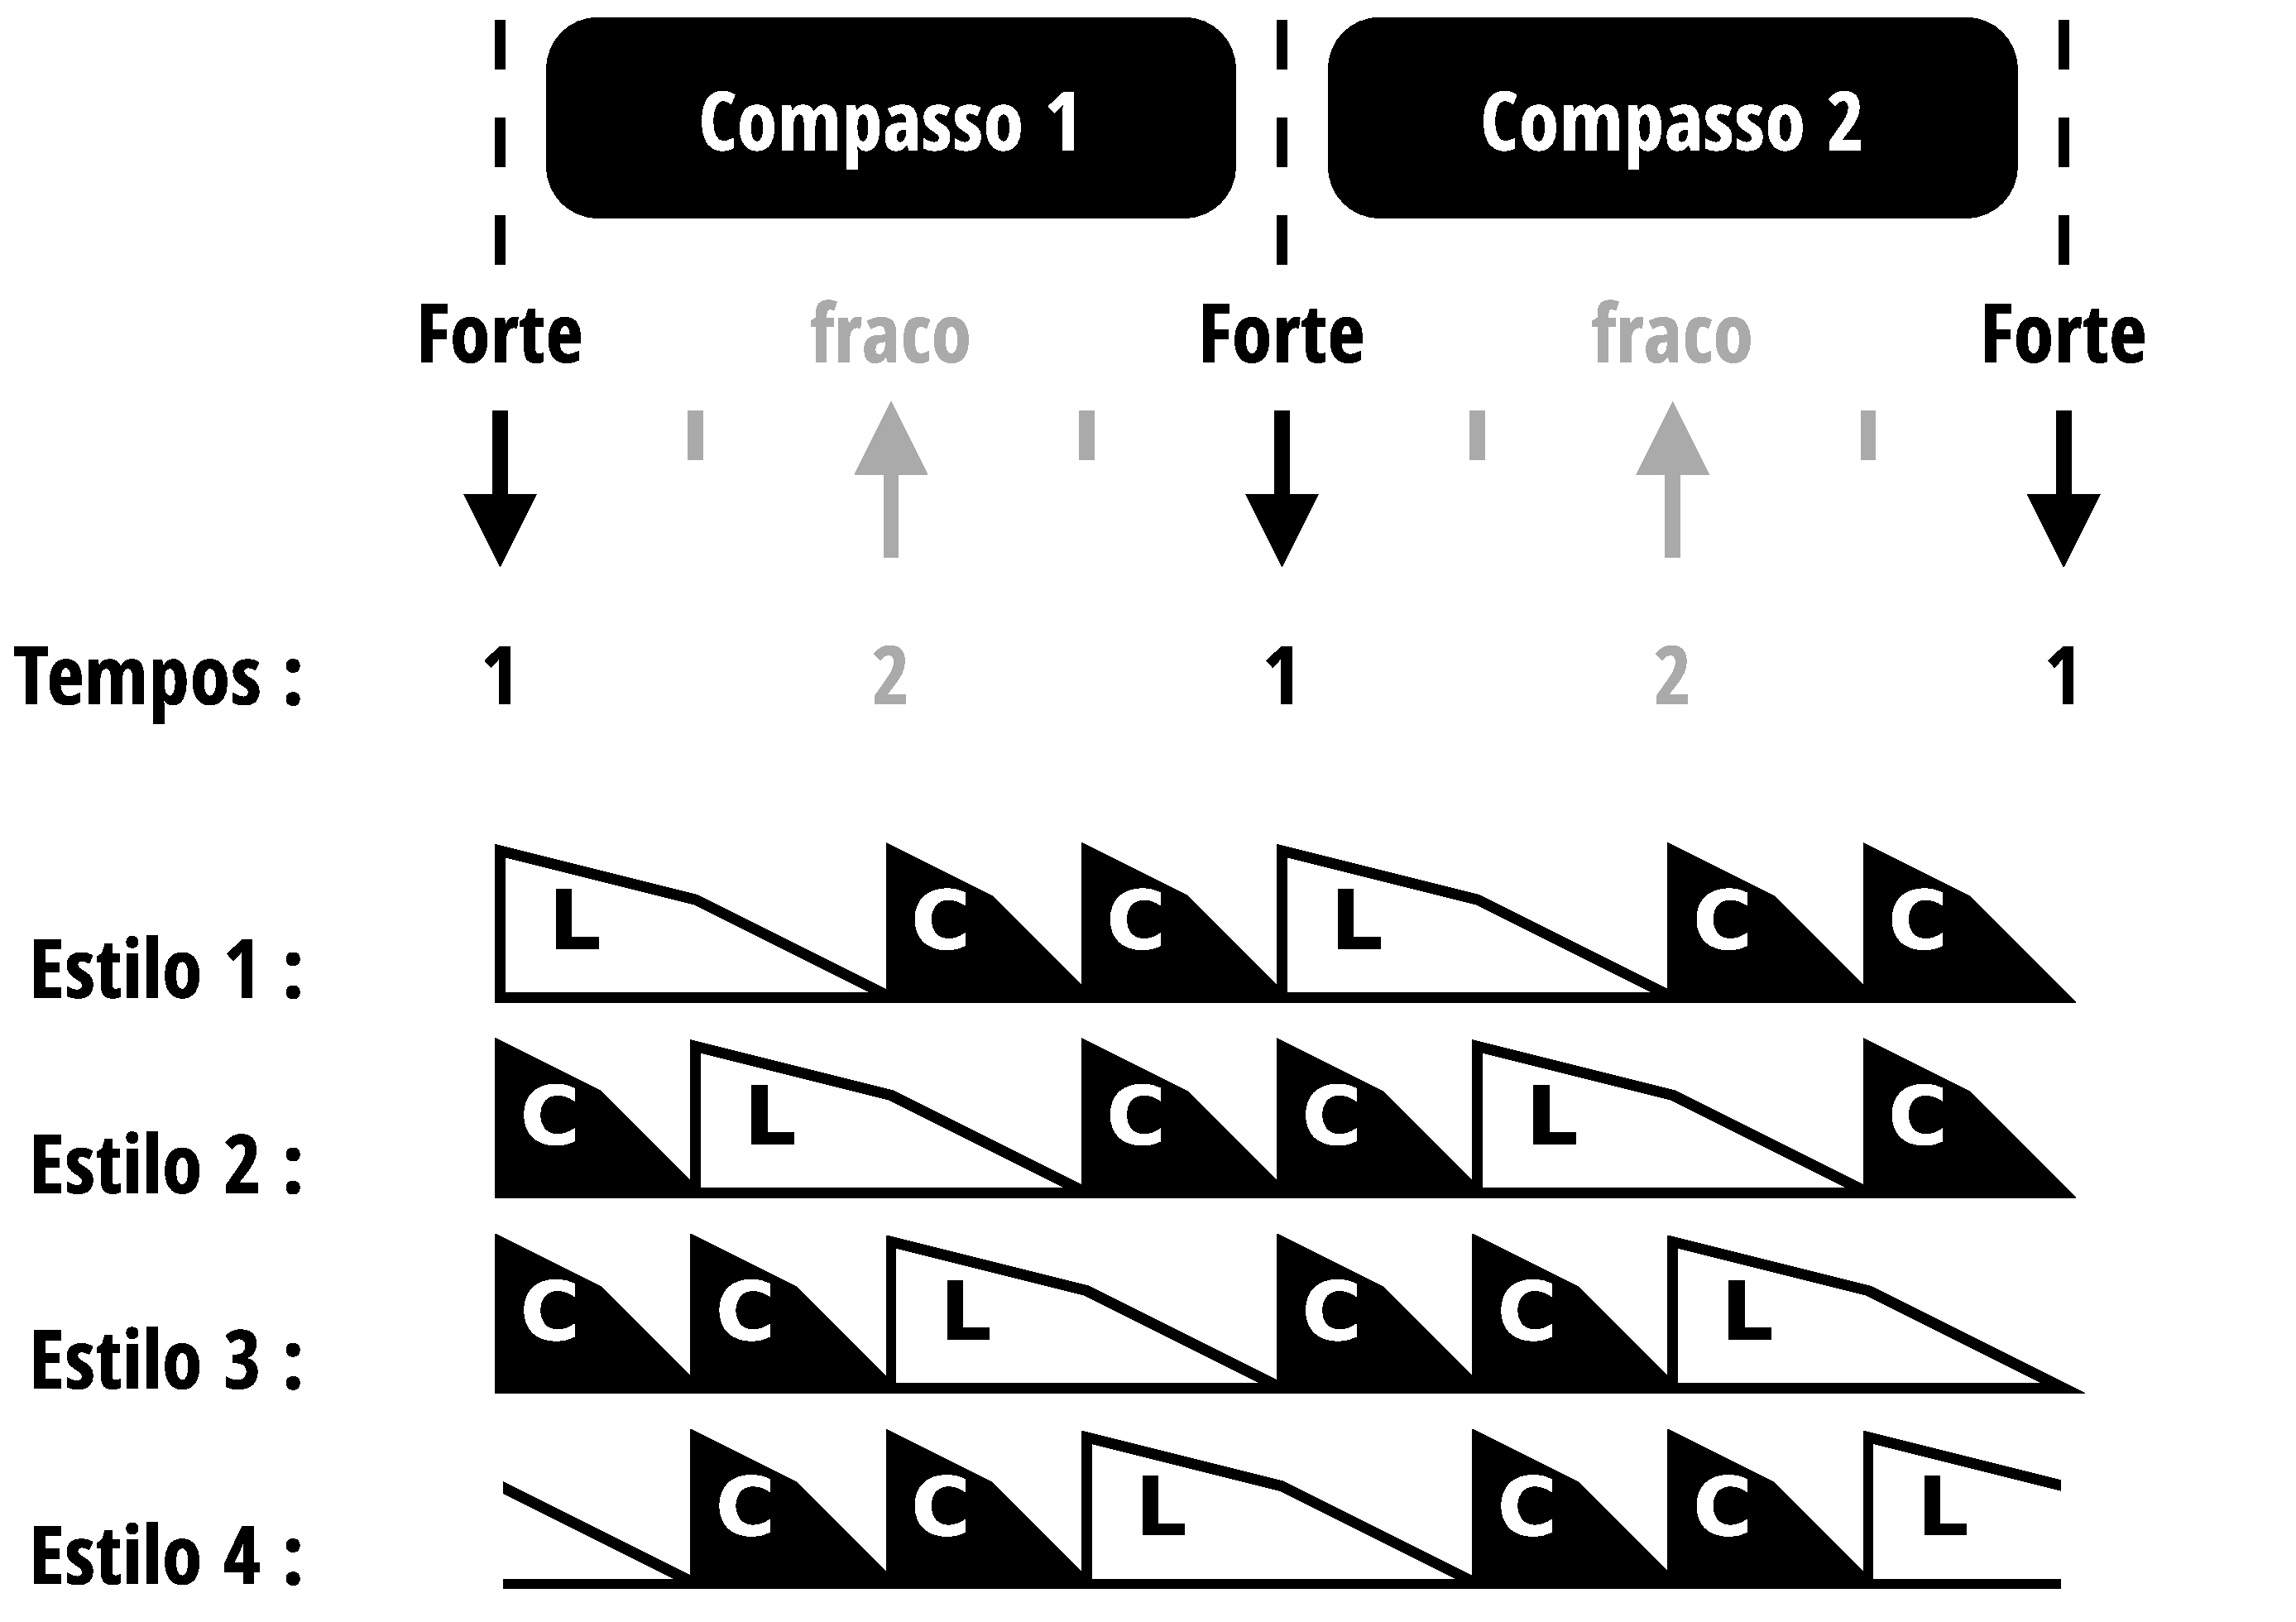
\includegraphics[width=0.5\textwidth]{chapters/cap-musicalidade/bailarcontratempo.eps}
    \caption{Dançando em tempo e contratempo.}\label{fig:tempovscontratempo}
\end{figure}




%%%%%%%%%%%%%%%%%%%%%%%%%%%%%%%%%%%%%%%%%%%%%%%%%%%%%%%%%%%%%%%%%%%%%%%%%%%%%%%%
\subsection{Que significa dançar em contratempo?}
Nesta seção presentaremos uma definição para o uso termo contratempo na dança,
este será diferente dos já mencionados na Seção \ref{subsec:contratempobrasil};
e terá afinidade  com os usos explicados nas 
Seções \ref{subsec:contratempoespanha} e \ref{subsec:contratempocuba},
que tem uma coerência maior com a \hyperref[sec:contratempo]{\textbf{acepção musical de contratempo}}.

A explicação já foi adiantada\footnote{Para 
ver a definição de dançar em contratempo ir a Pag. \pageref{def:DancaNoContratempo}.}
 na Definição \ref{def:DancaNoContratempo};
onde se menciona que para dançar a contratempo deve-se primeiro definir,
 qual é o movimento principal ou inicial do passo,
e logo executar esse movimento ao inicio de qualquer tempo fraco, ou parte fraca do tempo.

\begin{example}[Frente trás:]
Seguindo a definição do movimento descrita no Exemplo \ref{ex:frentetrasex},
sabe-se que o movimento longo é o primeiro;
assim, para dançar no contratempo, esse movimento deve ser encaixado num tempo fraco,
ou parte fraca do tempo.
Isto é mostrado nos Estilos 2, 3 e 4 da Figura \ref{fig:tempovscontratempo},
onde ``L'' representa o movimento com deslocamento longo,
e ``C'' representa o movimento sem deslocamento.
\begin{itemize} 
\item No ``Estilo 2'' o passo é executado na parte fraca do tempo forte.
\item No ``Estilo 3'' o passo é executado no tempo fraco.
\item No ``Estilo 4'' o passo é executado na parte fraca do tempo fraco.
\end{itemize}
\end{example}
%%%%%%%%%%%%%%%%%%%%%%%%%%%%%%%%%%%%%%%%%%%%%%%%%%%%%%%%%%%%%%%%%%%%%%%%%%%%%%%%
\subsection{Mudar entre dançar no tempo forte e em contratempo}
Se percebemos  que estamos dançando em contratempo e desejamos dançar no tempo forte,
podemos seguir as seguintes indicações para mudar o estilo de dança.
\begin{itemize}
\item Podemos executar um \hyperref[def:PassoAContratempo]{\textbf{passo a contratempo}}\footnote{ Para 
ver a definição de passo a contratempo ir a Pag. \pageref{def:PassoAContratempo}.},
o que provocará mudar nossa dança de dançar no tempo forte a dançar em contratempo.
\begin{example}[Passos a contratempo:]~
\begin{itemize}
\item Caminhada a contratempo.
\end{itemize}
\end{example}
\item Quando realizamos um movimento, interrompemos ele num tempo fraco 
para iniciar o próximo num tempo forte.
\begin{example}
Fazemos balaços um número impar de vezes.
\end{example}
\end{itemize}



